%% AB HIER COMMANDS
\renewcommand*{\headfont}{\normalfont}
\renewcommand{\familydefault}{\sfdefault}

\ifthenelse{\equal{\KopfzeileBlank}{true}}{
	\ifthenelse{\equal{\TYP}{Arbeitsblatt}}{
		\ihead{\FACH\ \KLASSE\\ \TYP}
		\chead{Datum: \rule[0ex]{3cm}{1pt}\\ \EINHEIT}
		\ohead{Name: \rule[0ex]{3cm}{1pt}\\ \thepage\ von ~\pageref{LastPage}}
	}
	{\ihead{\FACH\ \KLASSE\\ \TYP\ (\TIME)}
		\chead{Datum: \rule[0ex]{3cm}{1pt}\\ \EINHEIT}
		\ohead{Name: \rule[0ex]{3cm}{1pt}\\ \thepage\ von ~\pageref{LastPage}}
	}
}
	{
	\ifthenelse{\equal{\TYP}{Arbeitsblatt}}{
		\ihead{\FACH\ \KLASSE\ (\LEHRER)\\ \TYP}
		\chead{\DATUM\\ \EINHEIT}
		\ohead{Name: \rule[0ex]{3cm}{1pt}\\ \thepage\ von ~\pageref{LastPage}}
	}
	{\ihead{\FACH\ \KLASSE\ (\LEHRER)\\ \TYP\ (\TIME)}
		\chead{\DATUM\\ \EINHEIT}
		\ohead{Name: \rule[0ex]{3cm}{1pt}\\ \thepage\ von ~\pageref{LastPage}}
	}
	}

\ofoot{\ccLogo\ \ccAttribution\ \ccShareAlike\ \ccNonCommercialEU\ T. Tischler, \the\year{}}


%% Karierte Felder
\newcommand{\kariert}[2][1]{
	\begin{center}
		\begin{tikzpicture}
			\draw[step=0.5cm, color=gray] (0,0) grid (#1\linewidth,#2 cm);
		\end{tikzpicture}
	\end{center}
	}

%% Linien zum Schreiben
\newcounter{zeilen}
\newcounter{maxzeilen}
\newcommand{\liniert}[2][1]{
%	\addtocounter{maxzeilen}{#1}
	\setcounter{zeilen}{1}
	\setcounter{maxzeilen}{#2}
	\addtocounter{maxzeilen}{1}
	\
	\begin{center}
		\forloop{zeilen}{1}{\value{zeilen} < \value{maxzeilen}}{
	
			\rule{#1\linewidth}{1pt}
			}	
	\end{center}
	}
	
%% Für Punkte und Erwartungsbild am Ende
\newcounter{punkte}
\setcounter{punkte}{1}
\newcounter{erwartung}
\setcounter{erwartung}{1}
\newcounter{gesamt}
\setcounter{gesamt}{0}
\ifthenelse{\equal{\TYP}{Arbeitsblatt}}{
	\newcommand{\aufgabe}[1]{
		\addtocounter{subsection}{1}\subsection*{Aufgabe \the\value{subsection}: #1}
		}
	}
	{\newcommand{\aufgabe}[3]{
		\addtocounter{subsection}{1}\subsection*{Aufgabe \the\value{subsection}: #1 (#2 P.)}\addtocounter{gesamt}{#2}\expandafter\newcommand\csname punkteliste\the\value{punkte} \endcsname{#2}\stepcounter{punkte}\expandafter\newcommand\csname erwartungsliste\the\value{erwartung} \endcsname{#3}\stepcounter{erwartung}
		}
	}
\newcommand{\station}[1]{
	\addtocounter{section}{1}\section*{Station \the\value{section}: #1}
	}

%% Bruchdarstellung am Kreis
\newcommand*\kreisbruch[3][red]{%
	\vspace{0.5cm}
  \begin{tikzpicture}[baseline={(0,0)}]
    % Anteil färben:
    \fill[#1]
      % Linie:
      (0,0) -- ++(0:1cm)
      % anschließend Bogen entsprechend des Anteils:
      arc[start angle=0, delta angle=360/#3*#2,radius=1cm]
      % zurück zur Mitte:
      -- cycle ;
    % die Teile darüber zeichnen:
    \foreach \t in {1,...,#3} {
      \draw (0,0) -- ++(360/#3*\t:1cm) ;
    }
    % den ganzen Kreis darüber zeichnen:
    \draw (0,0) circle (1cm) ;    
  \end{tikzpicture}%
}

%% Bruchdarstellung am Rechteck
\newcommand{\rechteckbruch}[3][red]{
	\vspace{0.5cm}
	\begin{tikzpicture}
		\draw[draw=red, fill=#1] (0,0) rectangle ++(#2,2);
%		(0,0) -- ++(90:1cm)
		\foreach \r in {1,...,#3} {
			\draw (\r-1,0) rectangle ++(1,2) ;
		}
		\draw (0,0) rectangle ++(#3,2) ;
	\end{tikzpicture}
}

%% einzelne Funktion zeichnen
\newcommand{\funktion}[6]{
  \begin{tikzpicture}
    \begin{axis}[
      xmin=#2, xmax=#3,
      ymin=#4, ymax=#5,
      xlabel=$x$,
      ylabel=$y$,
      domain=#2:#3,
      samples=100,
      grid
    ]
      \addplot [#6] {#1};
      \node [#6] at (axis cs:#3-2,0.8*#5) {$f(x) = #1$};
    \end{axis}
  \end{tikzpicture}
}

%% Automatische leichte Matheaufgaben
%\definecolor{lightgray}{RGB}{220,220,220}
%
%\newcommand{\matheaufgaben}[2]{
%	\begin{tasks}[counter-format={(tsk[a])},label-offset=1em,after-item-skip=1em](\textwidth/4)
%	\foreach \x in {1,...,#1}{
%		\pgfmathrandominteger{\a}{1}{100}
%		\pgfmathrandominteger{\b}{1}{100}
%		\pgfmathrandominteger{\operator}{1}{3}
%		
%		\task Berechne $\a #2[\operator] \b$.
%		
%		\vspace{0.5em}
%		\begin{framed}
%			\colorbox{lightgray}{Ergebnis:} \underline{\hspace{3em}}
%		\end{framed}
%	}
%	\end{tasks}
%}

%% Lückentext
\newenvironment{LKtext}
{%
		\setlength{\baselineskip}{0.8cm}
	\newlength{\lkl}
	\newcommand{\lk}[1]{
	\ifthenelse{\equal{\LOSUNG}{true}}{
		\textit{##1}
	}{
		\settowidth{\lkl}{##1}
		\hspace*{-0.2\lkl}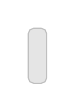
\begin{tikzpicture}[baseline={(0, -0.2)}, rounded corners=2pt]
			\node[draw=gray!50, fill=gray!20, minimum height=0.7cm, minimum width=2\lkl] {};
		\end{tikzpicture}\unskip
	}
	}
	\begin{adjustwidth}{0cm}{}\begin{list}{}{%
    \setlength{\leftmargin}{0cm}
  	}%
  	\item[]%
}{\end{list}\end{adjustwidth}}


%% Titel anpassen
\newcommand{\TITEL}{
	\begin{center}
	\Large
	\ifthenelse{\NOT\equal{\TYP}{Arbeitsblatt}}{
		\TYP\\
		\THEMA
	}{
	\THEMA
	}
	\end{center}
}